\documentclass[11pt,a4paper]{article}

% ============================================================
% Paquetes
% ============================================================
\usepackage[utf8]{inputenc}
\usepackage[T1]{fontenc}
\usepackage[spanish,es-tabla,es-noshorthands]{babel}
\decimalpoint
% Fallback manual para nombres en castellano si el paquete babel-spanish
% no está instalado. El \AtBeginDocument garantiza que estos
% renombramientos sobrescriban los de babel.
\AtBeginDocument{%
    \renewcommand{\figurename}{Figura}%
    \renewcommand{\tablename}{Tabla}%
    \renewcommand{\contentsname}{Índice}%
    \renewcommand{\refname}{Referencias}%
    \renewcommand{\bibname}{Bibliografía}%
    \renewcommand{\abstractname}{Resumen}%
    \renewcommand{\indexname}{Índice alfabético}%
    \renewcommand{\listfigurename}{Índice de figuras}%
    \renewcommand{\listtablename}{Índice de tablas}%
}
\usepackage[a4paper,margin=2.45cm]{geometry}
\usepackage{amsmath}
\usepackage{helvet}
\renewcommand{\familydefault}{\sfdefault}
\usepackage{microtype}
\usepackage{graphicx}
\usepackage{xcolor}
\usepackage{tikz}
\usepackage{booktabs}
\usepackage{tabularx}
\usepackage{array}
\usepackage{enumitem}
\usepackage{hyperref}
\usepackage{listings}
\usepackage{caption}
\captionsetup[table]{
	name = Tabla, format=plain, labelsep=newline,singlelinecheck=false, textfont=it, labelfont=bf
}

\captionsetup[figure]{
	format=plain, labelsep=newline,singlelinecheck=false, textfont=it, labelfont=bf
}
\usepackage{subcaption}
\usepackage{float}

\usetikzlibrary{positioning, shapes.geometric, arrows.meta, fit, backgrounds}

% ============================================================
% Colores del proyecto
% ============================================================
\definecolor{primario}{HTML}{3C3489}
\definecolor{secundario}{HTML}{0F6E56}
\definecolor{acento}{HTML}{BA7517}
\definecolor{grisClaro}{HTML}{F1EFE8}
\definecolor{grisTexto}{HTML}{444441}
\definecolor{codeBg}{HTML}{F7F6F1}
\definecolor{codeKey}{HTML}{3C3489}
\definecolor{codeComm}{HTML}{0F6E56}

% ============================================================
% Configuracion de hyperref
% ============================================================
\hypersetup{
    colorlinks=true,
    linkcolor=primario,
    urlcolor=primario,
    citecolor=primario,
    pdftitle={Avance 1 - Big Data Analysis},
    pdfauthor={Rios, Huaman, Merino, Montes},
}

% ============================================================
% Estilo de codigo SQL
% ============================================================
\lstdefinestyle{sqlstyle}{
    language=SQL,
    backgroundcolor=\color{codeBg},
    basicstyle=\ttfamily\footnotesize\color{grisTexto},
    keywordstyle=\color{codeKey}\bfseries,
    commentstyle=\color{codeComm}\itshape,
    stringstyle=\color{acento},
    showstringspaces=false,
    breaklines=true,
    frame=leftline,
    framerule=2pt,
    rulecolor=\color{primario},
    xleftmargin=10pt,
    aboveskip=10pt,
    belowskip=10pt,
    tabsize=2,
    morekeywords={VARCHAR, DECIMAL, TINYINT, SMALLINT, BIT, IDENTITY, CLUSTERED, NONCLUSTERED}
}
\lstset{style=sqlstyle}

% ============================================================
% Titulos de seccion con color
% ============================================================
\usepackage{titlesec}
\titleformat{\section}
    {\color{primario}\Large\bfseries}
    {\thesection.}{0.6em}{}
\titleformat{\subsection}
    {\color{secundario}\large\bfseries}
    {\thesubsection}{0.5em}{}

% ============================================================
% Captions
% ============================================================
\captionsetup{labelfont={bf,color=primario}, textfont=it, font=small}

% ============================================================
% Tabla de anchos flexibles
% ============================================================
\newcolumntype{L}[1]{>{\raggedright\arraybackslash}p{#1}}
\newcolumntype{C}[1]{>{\centering\arraybackslash}p{#1}}

% ============================================================
% INICIO DEL DOCUMENTO
% ============================================================
\begin{document}

% ------------------------------------------------------------
% Portada
% ------------------------------------------------------------
\begin{titlepage}
\centering
\vspace*{2cm}

{\color{primario}\rule{\textwidth}{1.5pt}}
\vspace{0.8cm}

{\Large\bfseries Big Data Analysis}\\[0.5cm]
{\Huge\bfseries\color{primario} Avance 1}\\[0.5cm]
{\Large Proyecto Olist: e-commerce brasileño\\ como caso de estudio para el mercado peruano}

\vspace{0.5cm}
{\color{primario}\rule{\textwidth}{1.5pt}}

\vspace{2.5cm}
{\large\bfseries Integrantes:}\\[0.6cm]

\begin{tabular}{l}
Rios Chiuca, Jaime Arturo\\[0.2cm]
Huaman Llanos, Felix Moises\\[0.2cm]
Merino Huaman, Manuel\\[0.2cm]
Montes Quispe, Adrian Guido\\
\end{tabular}

\vfill

{\large\bfseries Contenido del avance:}\\[0.3cm]
{\large KPIs del proyecto $\cdot$ Modelo conceptual $\cdot$ Modelo lógico $\cdot$ Modelo físico}

\vspace{1cm}
{\large Lima, \today}
\end{titlepage}

% ------------------------------------------------------------
% Introduccion breve
% ------------------------------------------------------------
\section*{Introducción}
\addcontentsline{toc}{section}{Introducción}

El presente avance responde a la primera entrega del proyecto de consultoría analítica sobre el dataset Olist Brazilian E-Commerce. El objetivo es definir la base de trabajo sobre la cual se construirán los análisis de los cinco problemas de negocio planteados: rentabilidad por categoría, retención de clientes, control de tiempos de entrega, desempeño de vendedores e identificación de causas de insatisfacción.

Toda la arquitectura de datos que se presenta a continuación: KPIs, modelos conceptual, lógico y físico, está diseñada con un criterio único: habilitar respuestas accionables a esos cinco problemas de negocio, no simplemente describir la estructura de los datos originales.

% ============================================================
% SECCION 1: KPIs
% ============================================================
\section{KPIs del proyecto}

Los indicadores clave de desempeño (KPIs) traducen las preguntas de la gerencia en métricas cuantificables. En lugar de presentarlos como una lista general del negocio, los organizamos por el problema al que responden, de forma que cada uno pueda rastrearse hasta una decisión concreta que la dirección debe tomar.

\subsection{KPIs agrupados por problema de negocio}

\renewcommand{\arraystretch}{1.3}

\newcommand{\kpiheader}[1]{%
    \vspace{0.6em}%
    \noindent{\color{primario}\textbf{#1}}\par
    \vspace{0.3em}%
}

\kpiheader{Problema 1 — Rentabilidad por categoría}
\noindent\begin{tabularx}{\textwidth}{@{}L{4cm} X L{2.3cm}@{}}
\toprule
\textbf{KPI} & \textbf{Fórmula} & \textbf{Unidad} \\
\midrule
Ingreso total & $\sum(\text{precio} + \text{flete})$ & R\$ \\
Ticket promedio & Ingreso total / número de pedidos & R\$ / pedido \\
Concentración de ingreso & \% ingreso del top 5 de categorías sobre el total & \% \\
Flete sobre precio & $(\text{flete} / \text{precio}) \times 100$ & \% \\
\bottomrule
\end{tabularx}

\kpiheader{Problema 2 — Retención de clientes}
\noindent\begin{tabularx}{\textwidth}{@{}L{4cm} X L{2.3cm}@{}}
\toprule
\textbf{KPI} & \textbf{Fórmula} & \textbf{Unidad} \\
\midrule
Tasa de recompra & Clientes con $\geq 2$ pedidos / total de clientes $\times 100$ & \% \\
Clientes únicos & Número de \texttt{customer\_unique\_id} distintos & Unidades \\
Valor de vida del cliente (CLV aproximado) & Ingreso total / clientes únicos & R\$ / cliente \\
Distribución RFM & Proporción de clientes por segmento (VIP, Frecuente, En riesgo, Dormido, Perdido) & \% \\
\bottomrule
\end{tabularx}

\kpiheader{Problema 3 — Control de tiempos de entrega}
\noindent\begin{tabularx}{\textwidth}{@{}L{4cm} X L{2.3cm}@{}}
\toprule
\textbf{KPI} & \textbf{Fórmula} & \textbf{Unidad} \\
\midrule
Porcentaje de entregas a tiempo & Pedidos con \texttt{dias\_retraso} $\leq 0$ / total de pedidos $\times 100$ & \% \\
Tiempo promedio de entrega & Promedio de \texttt{dias\_hasta\_entrega} & Días \\
Días de retraso promedio & Promedio de \texttt{dias\_retraso} sobre pedidos retrasados & Días \\
Pedidos con retraso crítico & \% de pedidos con \texttt{dias\_retraso} $> 7$ & \% \\
\bottomrule
\end{tabularx}

\kpiheader{Problema 4 — Desempeño de vendedores}
\noindent\begin{tabularx}{\textwidth}{@{}L{4cm} X L{2.3cm}@{}}
\toprule
\textbf{KPI} & \textbf{Fórmula} & \textbf{Unidad} \\
\midrule
Rating promedio por vendedor & Promedio de \texttt{puntuacion\_review} por \texttt{id\_vendedor} & 1 a 5 \\
Pedidos con problemas por vendedor & \% de pedidos del vendedor con puntuación $\leq 2$ & \% \\
Ingreso por vendedor & $\sum \text{valor\_total}$ agrupado por vendedor & R\$ \\
Vendedores críticos & \% de vendedores con rating $< 3.5$ y puntualidad $< 80\%$ & \% \\
\bottomrule
\end{tabularx}

\kpiheader{Problema 5 — Causas de insatisfacción}
\noindent\begin{tabularx}{\textwidth}{@{}L{4cm} X L{2.3cm}@{}}
\toprule
\textbf{KPI} & \textbf{Fórmula} & \textbf{Unidad} \\
\midrule
Porcentaje de reseñas positivas & Reseñas con puntuación 4-5 / total de reseñas $\times 100$ & \% \\
Porcentaje de reseñas negativas & Reseñas con puntuación 1-2 / total de reseñas $\times 100$ & \% \\
NPS estimado & \% promotores (5) $-$ \% detractores (1-2) & Puntos \\
Evolución de satisfacción & Promedio mensual de puntuación, serie de tiempo & 1 a 5 \\
\bottomrule
\end{tabularx}

\vspace{0.8em}
Los 21 indicadores definidos cubren las tres dimensiones clásicas del negocio, rentabilidad, cliente y operación; y a la vez responden punto por punto a las preguntas centrales del enunciado del proyecto. Todos se calculan directamente sobre las tablas del modelo que se presenta en las siguientes secciones, sin requerir transformaciones adicionales.

% ============================================================
% SECCION 2: Modelo conceptual
% ============================================================
\section{Modelo conceptual}

El modelo conceptual representa las entidades del negocio y las relaciones entre ellas, sin comprometerse todavía con detalles de implementación. En el caso de Olist, el sistema gira en torno a siete entidades: Cliente, Pedido, Producto, Vendedor, Pago, Reseña y Ubicación.

\subsection{Entidades y relaciones}

Un cliente puede realizar múltiples pedidos (relación $1:N$), y cada pedido contiene uno o varios ítems; cada ítem asocia a un producto con el vendedor que lo despacha, lo cual genera la relación $N:M$ entre pedidos y productos. Cada pedido tiene al menos una forma de pago asociada, y opcionalmente puede recibir una reseña por parte del cliente, por eso la relación entre Pedido y Reseña es $1:0..1$, no todos los pedidos generan reseña. Finalmente, tanto Cliente como Vendedor están vinculados a una Ubicación geográfica, lo cual es esencial para el análisis de rutas logísticas del Problema 3.

\begin{figure}[H]
\raggedright
\caption{Modelo conceptual del dominio Olist.}
\begin{tikzpicture}[
    node distance=1.6cm and 2.4cm,
    entidad/.style={
        rectangle,
        rounded corners=3pt,
        draw,
        line width=0.5pt,
        minimum width=2.4cm,
        minimum height=0.9cm,
        align=center,
        font=\small\bfseries,
    },
    cliente/.style={entidad, fill=secundario!15, draw=secundario},
    pedido/.style={entidad, fill=primario!15, draw=primario},
    producto/.style={entidad, fill=acento!20, draw=acento},
    vendedor/.style={entidad, fill=acento!30, draw=acento},
    pago/.style={entidad, fill=primario!8, draw=primario!70},
    resena/.style={entidad, fill=secundario!25, draw=secundario},
    ubic/.style={entidad, fill=grisClaro, draw=grisTexto},
    rel/.style={-{Latex[length=1.5mm]}, thick, color=grisTexto},
    cardi/.style={font=\footnotesize\itshape, color=grisTexto, inner sep=2pt, fill=white},
]

\node[ubic]     (ubic)     at ( 0,  0)  {Ubicación};
\node[cliente]  (cliente)  at ( 0, -2)  {Cliente};
\node[pedido]   (pedido)   at ( 5, -2)  {Pedido};
\node[producto] (producto) at (10, -2)  {Producto};
\node[vendedor] (vendedor) at (10,  0)  {Vendedor};
\node[pago]     (pago)     at ( 5, -4)  {Pago};
\node[resena]   (resena)   at ( 0, -4)  {Reseña};

\draw[rel] (cliente)  -- node[cardi] {$1 : N$}    (pedido);
\draw[rel] (pedido)   -- node[cardi] {$N : M$}    (producto);
\draw[rel] (cliente)  -- node[cardi] {$N : 1$}    (ubic);
\draw[rel] (vendedor) -- node[cardi] {$N : 1$}    (producto);
\draw[rel] (vendedor.west) -- node[cardi, pos=0.6] {$N : 1$} (ubic.east);
\draw[rel] (pedido)   -- node[cardi] {$1 : N$}    (pago);
\draw[rel] (pedido)   -- node[cardi] {$1 : 0..1$} (resena);

\end{tikzpicture}
\label{fig:conceptual}
\end{figure}

\subsection{Decisiones clave del modelo conceptual}

\begin{itemize}[leftmargin=*, itemsep=2pt]
    \item La entidad \textbf{Ubicación} se incluye explícitamente (no como atributo de Cliente o Vendedor) porque interviene en dos problemas de negocio distintos: análisis regional del cliente (Problema 2) y construcción de rutas logísticas origen$\to$destino (Problema 3).
    \item La relación Pedido-Reseña es $1:0..1$ y no $1:1$: solo una parte de los pedidos genera reseña, y ese subconjunto es el que alimenta los KPIs de satisfacción del Problema 5.
    \item La relación Producto-Vendedor es $N:1$ dentro de cada ítem del pedido, un producto se despacha desde un único vendedor en una transacción específica, pero el mismo producto puede ser ofrecido por varios vendedores distintos a través del tiempo.
\end{itemize}

% ============================================================
% SECCION 3: Modelo logico
% ============================================================
\section{Modelo lógico}

El modelo lógico traduce las entidades conceptuales a una arquitectura orientada al análisis multidimensional. Se optó por un \textbf{modelo en estrella}, donde una tabla central de hechos \texttt{FACT\_VENTAS} se conecta a seis dimensiones que permiten filtrar, agrupar y pivotar la información según distintas perspectivas de negocio.

\subsection{Granularidad de la tabla de hechos}

El grano de \texttt{FACT\_VENTAS} es el \textbf{ítem vendido}, no el pedido. Esta decisión es importante: un pedido puede contener productos de múltiples categorías y vendedores distintos, por lo que si el grano fuera el pedido se perdería la capacidad de analizar rentabilidad por categoría (Problema 1) y desempeño por vendedor (Problema 4). Con el grano a nivel de ítem, cada línea de la tabla representa un producto comprado por un cliente, despachado por un vendedor, en una fecha específica.

\subsection{Diagrama del modelo estrella}

\begin{figure}[H]
\raggedright
\caption{Modelo en estrella: tabla de hechos y seis dimensiones.}
\begin{tikzpicture}[
    node distance=2cm,
    fact/.style={
        rectangle,
        rounded corners=4pt,
        draw=primario,
        line width=0.8pt,
        fill=primario!15,
        minimum width=4cm,
        minimum height=2cm,
        align=center,
        font=\small\bfseries,
    },
    dim/.style={
        rectangle,
        rounded corners=3pt,
        draw=secundario,
        line width=0.5pt,
        fill=secundario!15,
        minimum width=2.8cm,
        minimum height=0.9cm,
        align=center,
        font=\small\bfseries,
    },
    link/.style={-{Latex[length=1.8mm]}, thick, color=primario},
]

\node[fact] (fact) at (0,0) {FACT\_VENTAS\\[2pt]\footnotesize\normalfont\itshape Grano: ítem vendido};

\node[dim] (tiempo)    at ( -5,   2.2) {DIM\_TIEMPO};
\node[dim] (cliente)   at (  5,   2.2) {DIM\_CLIENTE};
\node[dim] (producto)  at ( -5,   0)   {DIM\_PRODUCTO};
\node[dim] (vendedor)  at (  5,   0)   {DIM\_VENDEDOR};
\node[dim] (pago)      at ( -5,  -2.2) {DIM\_PAGO};
\node[dim] (geografia) at (  5,  -2.2) {DIM\_GEOGRAFIA};

\draw[link] (tiempo)    -- (fact);
\draw[link] (cliente)   -- (fact);
\draw[link] (producto)  -- (fact);
\draw[link] (vendedor)  -- (fact);
\draw[link] (pago)      -- (fact);
\draw[link] (geografia) -- (fact);

\end{tikzpicture}
\label{fig:estrella}
\end{figure}

\subsection{Dimensiones y sus atributos}

\begin{tabularx}{\textwidth}{@{}L{3.2cm} X@{}}
\toprule
\textbf{Tabla} & \textbf{Contenido y propósito} \\
\midrule
\texttt{FACT\_VENTAS} & Una fila por ítem vendido. Contiene las métricas cuantitativas del negocio: precio, flete, valor total, días hasta entrega, días de retraso, flag de entrega a tiempo, flete sobre precio, puntuación de reseña, nivel de satisfacción y flag de comentario escrito. \\
\addlinespace
\texttt{DIM\_TIEMPO} & Descomposición de la fecha en año, mes, trimestre, día de la semana y flag de fin de semana. Permite análisis temporales y estacionales (Problemas 1 y 3). \\
\addlinespace
\texttt{DIM\_CLIENTE} & Identificador del cliente y su \texttt{customer\_unique\_id} (necesario para calcular recompra). Enlaza a \texttt{DIM\_GEOGRAFIA} para el análisis regional. \\
\addlinespace
\texttt{DIM\_PRODUCTO} & Categoría del producto traducida al español, rango de precio (bajo/medio/alto), peso y dimensiones. Base del Problema 1. \\
\addlinespace
\texttt{DIM\_VENDEDOR} & Identificador del vendedor y su ubicación geográfica. Base del Problema 4. \\
\addlinespace
\texttt{DIM\_PAGO} & Tipo de pago y número de cuotas. Permite cruzar comportamiento financiero con rentabilidad (Problema 1). \\
\addlinespace
\texttt{DIM\_GEOGRAFIA} & Dimensión compartida (role-playing): se conecta dos veces a la tabla de hechos, una para la ubicación del cliente y otra para la ubicación del vendedor. Esto permite construir el análisis de rutas logísticas origen$\to$destino del Problema 3. \\
\bottomrule
\end{tabularx}

\subsection{Variables derivadas calculadas en el ETL}

Además de los campos originales de los nueve archivos CSV del dataset, el proceso de ETL genera las siguientes variables derivadas, que se materializan directamente como columnas de \texttt{FACT\_VENTAS}:

\begin{itemize}[leftmargin=*, itemsep=1pt]
    \item \texttt{valor\_total} = precio + flete
    \item \texttt{dias\_hasta\_entrega} = fecha\_entrega\_real $-$ fecha\_compra
    \item \texttt{dias\_retraso} = fecha\_entrega\_real $-$ fecha\_entrega\_estimada
    \item \texttt{entrego\_a\_tiempo} = 1 si \texttt{dias\_retraso} $\leq 0$, 0 en caso contrario
    \item \texttt{flete\_sobre\_precio} = (flete / precio) $\times$ 100
    \item \texttt{satisfaccion} = ``Buena'' (4-5), ``Regular'' (3), ``Mala'' (1-2)
    \item \texttt{escribio\_comentario} = 1 si el campo \texttt{review\_comment\_message} es no nulo, 0 en caso contrario
\end{itemize}

Materializar estas variables en la tabla de hechos (en lugar de calcularlas al vuelo en cada consulta) simplifica el trabajo del dashboard y garantiza consistencia entre vistas.

% ============================================================
% SECCION 4: Modelo fisico
% ============================================================
\section{Modelo físico}

El modelo físico lleva el diseño lógico a una implementación concreta sobre SQL Server. Se definen los tipos de datos, las claves primarias y foráneas, y los índices que optimizan las consultas más frecuentes del dashboard.

\subsection{Diagrama del modelo físico}

\begin{figure}[H]
\centering
\caption{Modelo físico: tablas, columnas, tipos de datos, claves primarias y foráneas.}
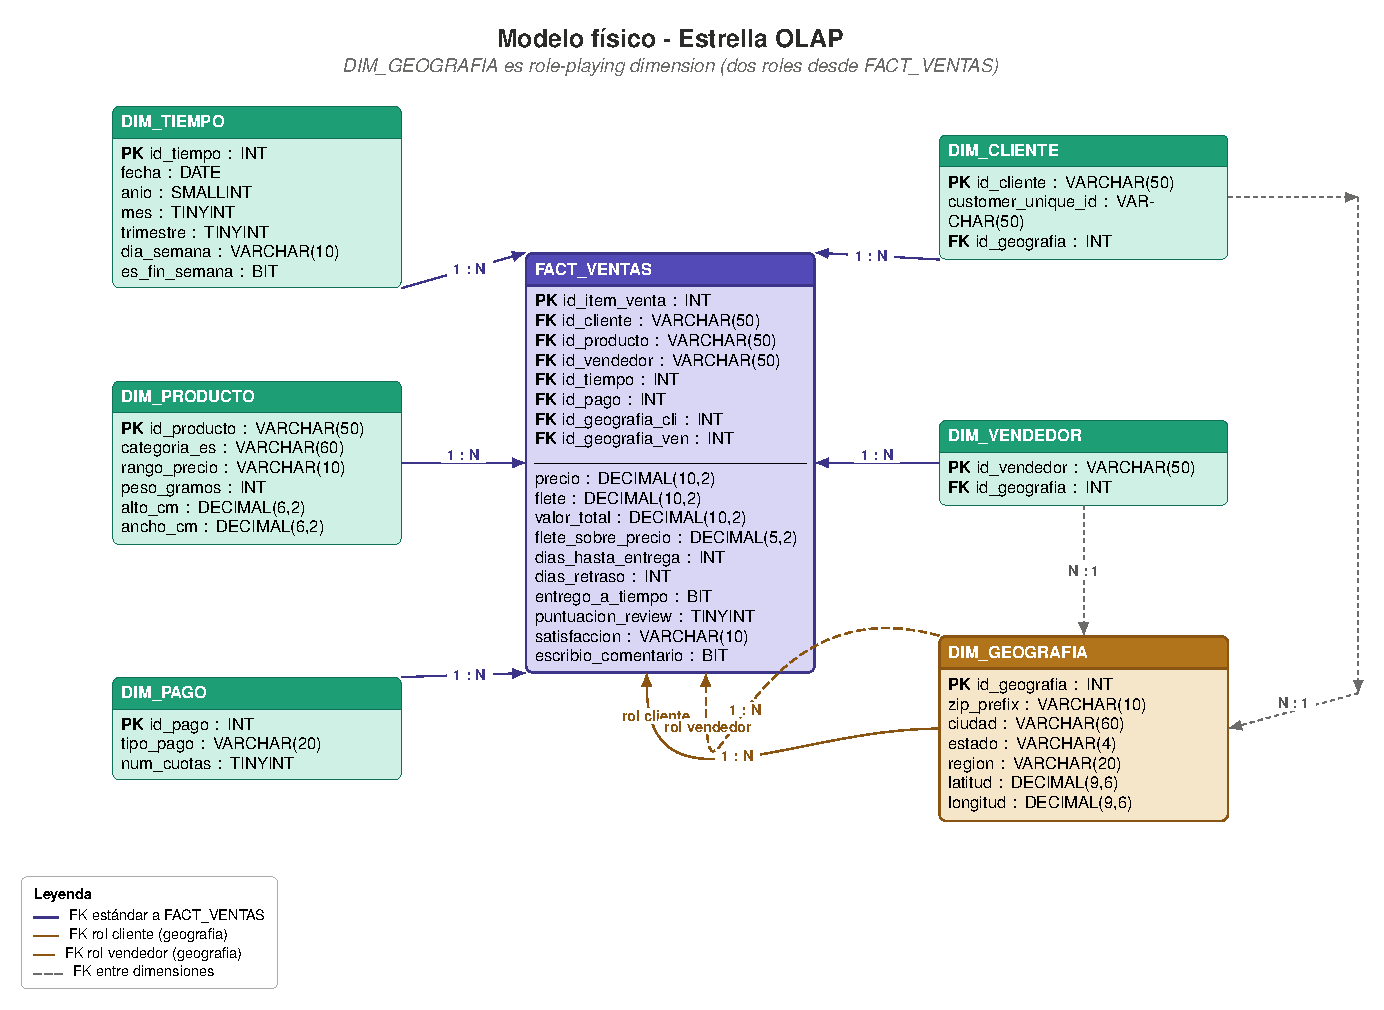
\includegraphics[width=\textwidth]{figuras/modelo_fisico_mejorado.pdf}

\label{fig:fisico}
\end{figure}

\subsection{Criterios de diseño físico}

\begin{itemize}[leftmargin=*, itemsep=2pt]
    \item \textbf{Tipos de datos ajustados al rango esperado.} Se usa \texttt{TINYINT} para valores de 0 a 255 (puntuación de reseña, número de cuotas, mes, trimestre), \texttt{SMALLINT} para el año, \texttt{BIT} para banderas booleanas (\texttt{entrego\_a\_tiempo}, \texttt{escribio\_comentario}, \texttt{es\_fin\_semana}) y \texttt{DECIMAL(10,2)} para valores monetarios.
    \item \textbf{Índices en columnas de filtrado frecuente.} Se definen índices secundarios sobre \texttt{id\_tiempo}, \texttt{id\_producto} y \texttt{id\_vendedor} en la tabla de hechos, que son los tres filtros más usados por el dashboard del Problema 1, 3 y 4 respectivamente.
    \item \textbf{Doble conexión a la dimensión geografía.} La tabla de hechos referencia \texttt{DIM\_GEOGRAFIA} dos veces: una por el lado del cliente (\texttt{id\_geografia\_cli}) y otra por el lado del vendedor (\texttt{id\_geografia\_ven}). Esta técnica de role-playing es la que permite construir las rutas origen$\to$destino del análisis logístico.
\end{itemize}

\subsection{Definición en SQL (DDL)}

A continuación se presenta el script completo de creación de las seis tablas del modelo. 
Está diseñado para SQL Server, pero es fácilmente portable a PostgreSQL o MySQL con 
ajustes menores de sintaxis.

El modelo es predominantemente en estrella, con una  concesión deliberada al copo de nieve en \texttt{DIM\_GEOGRAFIA}: tanto \texttt{DIM\_CLIENTE}  como \texttt{DIM\_VENDEDOR} tienen llave foránea hacia ella. Este patrón se conoce como  \emph{starflake}. Lo elegimos porque la información geográfica es compartida entre cliente  y vendedor, y duplicarla en ambas dimensiones sería redundancia sin valor analítico. Las  consultas críticas que cruzan geografía (rutas origen$\to$destino del Problema 3) pasan  directamente por \texttt{FACT\_VENTAS} mediante role-playing, así que el join adicional  desde las dimensiones de cliente o vendedor solo ocurre en consultas marginales.

\begin{lstlisting}[caption={Creacion de las tablas de dimensiones.}]
	-- Dimension TIEMPO
	-- Sin IDENTITY: la PK se carga con clave inteligente formato YYYYMMDD,
	-- lo cual permite filtrar rangos de fechas sin join con la dimension.
	CREATE TABLE DIM_TIEMPO (
	id_tiempo       INT           NOT NULL PRIMARY KEY,
	fecha           DATE          NOT NULL,
	anio            SMALLINT      NOT NULL,
	mes             TINYINT       NOT NULL,
	trimestre       TINYINT       NOT NULL,
	dia_semana      VARCHAR(10)   NOT NULL,
	es_fin_semana   BIT           NOT NULL
	);
	
	-- Dimension GEOGRAFIA (compartida entre cliente y vendedor)
	-- Surrogate key con IDENTITY porque el dataset no provee identificador propio.
	-- Restriccion UNIQUE para garantizar que cada combinacion geografica sea unica.
	CREATE TABLE DIM_GEOGRAFIA (
	id_geografia    INT           IDENTITY(1,1) PRIMARY KEY,
	zip_prefix      VARCHAR(10)   NOT NULL,
	ciudad          VARCHAR(60),
	estado          VARCHAR(4)    NOT NULL,
	region          VARCHAR(20)   NOT NULL,
	latitud         DECIMAL(9,6),
	longitud        DECIMAL(9,6),
	CONSTRAINT uq_geografia UNIQUE (zip_prefix, ciudad, estado)
	);
	
	-- Dimension CLIENTE
	-- PK preserva el id_cliente original del dataset Olist (trazabilidad).
	-- customer_unique_id es el identificador del cliente a traves del tiempo,
	-- critico para el calculo de retencion del Problema 2.
	-- FK a DIM_GEOGRAFIA: starflake deliberado para evitar duplicar geografia.
	CREATE TABLE DIM_CLIENTE (
	id_cliente          VARCHAR(50)   NOT NULL PRIMARY KEY,
	customer_unique_id  VARCHAR(50)   NOT NULL,
	id_geografia        INT           NOT NULL,
	FOREIGN KEY (id_geografia) REFERENCES DIM_GEOGRAFIA(id_geografia)
	);
	
	-- Dimension VENDEDOR
	-- FK a DIM_GEOGRAFIA por la misma razon que DIM_CLIENTE.
	CREATE TABLE DIM_VENDEDOR (
	id_vendedor     VARCHAR(50)   NOT NULL PRIMARY KEY,
	id_geografia    INT           NOT NULL,
	FOREIGN KEY (id_geografia) REFERENCES DIM_GEOGRAFIA(id_geografia)
	);
	
	-- Dimension PRODUCTO
	-- categoria_es ya viene traducida del portugues durante el ETL.
	-- rango_precio se discretiza en bajo / medio / alto para analisis ejecutivo.
	CREATE TABLE DIM_PRODUCTO (
	id_producto     VARCHAR(50)   NOT NULL PRIMARY KEY,
	categoria_es    VARCHAR(60),
	rango_precio    VARCHAR(10),
	peso_gramos     INT,
	alto_cm         DECIMAL(6,2),
	ancho_cm        DECIMAL(6,2)
	);
	
	-- Dimension PAGO
	-- Surrogate key con IDENTITY: el dataset solo provee tipo y cuotas,
	-- no un identificador unico de combinacion.
	CREATE TABLE DIM_PAGO (
	id_pago         INT           IDENTITY(1,1) PRIMARY KEY,
	tipo_pago       VARCHAR(20)   NOT NULL,
	num_cuotas      TINYINT       NOT NULL
	);
\end{lstlisting}

\begin{lstlisting}[caption={Creacion de la tabla de hechos y sus indices.}]
	-- Tabla de hechos FACT_VENTAS
	-- Granularidad: un item vendido (no un pedido), para preservar la informacion
	-- de categoria y vendedor cuando un pedido tiene productos heterogeneos.
	--
	-- Llaves foraneas:
	--   - 5 FK estandar a las dimensiones (cliente, producto, vendedor, tiempo, pago)
	--   - 2 FK a DIM_GEOGRAFIA (role-playing: rol cliente y rol vendedor)
	--
	-- Variables derivadas (calculadas en el ETL y materializadas):
	--   valor_total, flete_sobre_precio, dias_hasta_entrega, dias_retraso,
	--   entrego_a_tiempo, satisfaccion, escribio_comentario.
	CREATE TABLE FACT_VENTAS (
	id_item_venta       INT           IDENTITY(1,1) PRIMARY KEY,
	id_cliente          VARCHAR(50)   NOT NULL,
	id_producto         VARCHAR(50)   NOT NULL,
	id_vendedor         VARCHAR(50)   NOT NULL,
	id_tiempo           INT           NOT NULL,
	id_pago             INT           NOT NULL,
	id_geografia_cli    INT           NOT NULL,
	id_geografia_ven    INT           NOT NULL,
	precio              DECIMAL(10,2) NOT NULL,
	flete               DECIMAL(10,2) NOT NULL,
	valor_total         DECIMAL(10,2) NOT NULL,
	flete_sobre_precio  DECIMAL(5,2),
	dias_hasta_entrega  INT,
	dias_retraso        INT,
	entrego_a_tiempo    BIT,
	puntuacion_review   TINYINT,
	satisfaccion        VARCHAR(10),
	escribio_comentario BIT,
	FOREIGN KEY (id_cliente)       REFERENCES DIM_CLIENTE(id_cliente),
	FOREIGN KEY (id_producto)      REFERENCES DIM_PRODUCTO(id_producto),
	FOREIGN KEY (id_vendedor)      REFERENCES DIM_VENDEDOR(id_vendedor),
	FOREIGN KEY (id_tiempo)        REFERENCES DIM_TIEMPO(id_tiempo),
	FOREIGN KEY (id_pago)          REFERENCES DIM_PAGO(id_pago),
	FOREIGN KEY (id_geografia_cli) REFERENCES DIM_GEOGRAFIA(id_geografia),
	FOREIGN KEY (id_geografia_ven) REFERENCES DIM_GEOGRAFIA(id_geografia)
	);
	
	-- Indices secundarios sobre las columnas de filtrado mas frecuente del dashboard.
	-- No se indexan todas las FK porque cada indice acelera lectura pero penaliza
	-- escritura; solo se paga ese costo donde el dashboard realmente lo aprovecha.
	CREATE NONCLUSTERED INDEX idx_fact_tiempo
	ON FACT_VENTAS(id_tiempo);
	CREATE NONCLUSTERED INDEX idx_fact_producto
	ON FACT_VENTAS(id_producto);
	CREATE NONCLUSTERED INDEX idx_fact_vendedor
	ON FACT_VENTAS(id_vendedor);
\end{lstlisting}

\subsection{Decisiones de tipos de datos}

Cada tipo se ajustó al rango esperado de valores. \texttt{TINYINT} (0-255) se usó para 
puntuaciones, meses, trimestres y número de cuotas, ahorrando espacio frente a \texttt{INT}. 
\texttt{SMALLINT} para el año, suficiente hasta el año 32.767. \texttt{BIT} para flags 
booleanos como \texttt{entrego\_a\_tiempo} o \texttt{es\_fin\_semana}, que ocupan un solo 
bit en lugar de cuatro bytes. \texttt{DECIMAL(10,2)} para valores monetarios garantiza 
precisión sin pérdida por aritmética flotante. \texttt{DECIMAL(9,6)} para coordenadas 
geográficas mantiene precisión submétrica.

Las llaves naturales del dataset Olist (\texttt{id\_cliente}, \texttt{id\_producto}, 
\texttt{id\_vendedor}) se preservaron como \texttt{VARCHAR(50)} para mantener trazabilidad 
con los archivos fuente, evitando un paso adicional de mapeo en el ETL. Las dimensiones 
generadas por nosotros (\texttt{DIM\_GEOGRAFIA}, \texttt{DIM\_PAGO}) usan surrogate keys 
enteras con \texttt{IDENTITY(1,1)}, lo cual acelera los joins y reduce el espacio de la 
tabla de hechos.

\end{document}
